\chapter{Caracterizaci\'on de la emisi\'on de radio en eventos ES}
\label{ch:caracterizacionRadio}

En este cap\'itulo se realiza un recuento de las caracter\'isticas principales de la se\~nal de radio generada por lluvias ES.
Esto permitir\'a determinar el espacio de par\'ametros (energ\'ia, \'angulo cenital, etc) en el que este tipo de eventos prodr\'an ser detectados, y que por ende deber\'an ser simulados.

Para que un evento ES sea identificado como tal, es necesario que se cumplan dos condiciones:
\begin{enumerate}
 \item La se\~nal de radio a nivel del suelo deber\'a ser lo suficientemente intensa y extensa para disparar varias antenas del detector, es decir, debe ser capaz de satisfacer ciertos criterios de disparo locales y globales.
 \item Las caracter\'isticas globales del evento deben permitir distinguirlo de los eventos de fondo, que al igual que en Auger ser\'an los generados por lluvias hadr\'onicas iniciadas cerca del tope de la atm\'osfera.
\end{enumerate}
Por este motivo en la subsiguiente caracterizaci\'on, adem\'as de presentar las caracter\'isticas principales de la se\~nal generada por eventos ES, se har\'a incapi\'e en determinar en qu\'e regi\'on del espacio de par\'ametros las condiciones 1 y 2 se cumplen.

	\section{Caracter\'isticas generales: evento típico}
	
	El primer paso en la caracterizaci\'on de la emisión de radio de eventos ES ser\'a estudiar lo que denominaremos un \emph{evento típico} o \emph{de referencia}, cuyas caracter\'isticas ser\'an utilizadas como punto de comparaci\'on al variar los parametros de la simulaci\'on. 
	A saber, las cualidades que definen la emisi\'on de radio de una lluvia ES en este an\'alisis son: 
	\begin{itemize}
	 \item el canal de decaimiento del \tauon{};
	 \item la energía transferida a la lluvia $E_v$, o energ\'ia visible\footnote{Se denomina energ\'ia visible de la lluvia a la acarreada por las part\'iculas interactuantes en del decaimiento del \tauon{}, es decir, la que portan electrones, positrones, fotones y hadrones cargados.};
% 	 ue ser\'a transmitida r\'apidamente a las nuevas generaciones de part\'iculas. Por otro lado, la energ\'ia transferida a part\'iculas penetrantes, neutrinos y muones, se perder\'a debido a su baja frecuencia de interacci\'on.};
	 \item sus parámetros geométricos $(\theta,{\rm x_d},\phi)$;
	 \item la disposici\'on de las antenas;
	 \item la ubicaci\'on geogr\'afica del detector, que determina el campo geomagn\'etico.
	 
	\end{itemize}

	Es interesante destacar que a diferencia del calculo realizado en la primer parte de esta tesis, aqu\'i las lluvias ES se caracterizarán por su energía visible $E_v$ y no por la energía del \tauon{} emergente.
	Esto es una elecci\'on que en ciertas condiciones disminuye la cantidad de simulaciones que deben realizarse (ver secci\'on \ref{sbsc:decayChRadio}), aunque debe ser incluida correctamente al calcular la exposición del detector.
	
	Los par\'ametros del evento elegido como referencia se muestran en la tabla \ref{tab:paramTestShower}.
	%
	\begin{table}[ht!]
	 \begin{center}
	  \begin{tabular}{|c|cccc|}
	   \hline
	   Canal de decaimiento & $E_v$ & $\theta$ & \xd{} & $\phi$ \\
	   \hline
	   $\tau\rightarrow e^- \nu_{e^-}\nu\tau$ & \cant{10^{18}}{eV} & \cant{90.5}{^\circ} & \cant{25}{m} & \cant{90}{^\circ} \\
	   \hline
	  \end{tabular}
	  \caption{\label{tab:paramTestShower}
	  Parámetros de simulación del \emph{evento típico} que se utilizará como referencia.
	  }
	 \end{center}
	\end{table}
	%
	
	Para estudiar este evento se simular\'a su se\~nal sobre un arreglo de antenas cuyo paso es \cant{1000}{m} en la dirección de propagación y \cant{100}{m} en la dirección transversal, y cuyo tama\~no es \cant{2\times80}{km}.
	Estos par\'ametros, que no tendr\'an nada que ver con la disposici\'on de las antenas del detector real, representan una buena relaci\'on de compromiso entre la granularidad con la que se mide la se\~nal y los recursos de c\'omputo utilizados en cada evento.
	
	Dado que el campo geomagn\'etico afecta significativamente la se\~nal, es necesario definir tambi\'en la ubicaci\'on del detector. 
	Como ya se ha mencionado, el c\'alculo descripto en esta parte de la tesis no esta ligado a ning\'un experimento en particular, sin embargo, para elegir el sitio en el que se simular\'a el detector se consideraron s\'olo ubicaciones en las que ya se encuentre funcionando alg\'un experimento de rayos c\'osmicos que utilice la t\'ecnica de radio.
	Entonces, las locaciones tenidas en cuenta se detallan en la tabla \ref{tab:possibleLoc} junto con las caracter\'isticas del campo geomagn\'etico promedio en sus inmediaciones (datos tomados de \cite{noaa}).
	%
	\begin{table}[ht!]
	\centering
	\footnotesize
	\newcolumntype{L}{>{\centering\arraybackslash}m{2.25cm}}
		\begin{tabular}{LLLLL}
		\toprule
		Experimento (Sitio) & Coordenadas & Declinaci\'on (+E,-W) & Inclinaci\'on (+D,-U)& Intensidad [Gauss] \\
		\midrule
		PAO Aera (Malarg\"ue Argentina) 
		& $35^\circ12$'${\rm S} $ $69^\circ18$'${\rm W}$
		& $(1.68\pm0.37)^\circ$ & $-36.3\pm0.22)^\circ$ & $0.2392\pm0.0015$ \\ \midrule
		Tunka Rex  (Tunka Valley Rusia) 
		& $51^\circ48$'${\rm N}$ $103^\circ04$'${\rm E}$
		& $(-2.82\pm0.37)^\circ$ & $(-71.2\pm0.22)^\circ$ & $0.6037\pm0.0015$ \\ \midrule
		Trend  (Tian shan China) 
		& $40^\circ32$'${\rm N}$ $78^\circ25$'${\rm E}$
		& $(3.76\pm0.37)^\circ$ & $(60.0\pm0.22)^\circ$ & $0.5391\pm0.0015$ \\
		\bottomrule
		\end{tabular}
		\caption{\label{tab:possibleLoc} Ubicaciones consideradas para simular el detector, junto a las caracter\'isticas del campo geomagn\'etico~\cite{noaa}. Por su intensidad e inclinaci\'on, Tunka presenta el campo m\'as favorable para la detecci\'on de lluvias atmosf\'ericas inclinadas mediante t\'ecnicas de radio.}
	\end{table}
	
	De las tres posibles ubicaciones, Tunka posee el campo geomagn\'etico m\'as intenso y vertical\footnote{La inclinaci\'on presentada en la tabla \ref{tab:possibleLoc} es medida respecto del plano del suelo.}. 
	Dado que el impacto del efecto geomagn\'etico depende del producto $\vec{\beta}\times\vec{B}$, ambas cualidades favorecen la detecci\'on de eventos inclinados.
	Por este motivo el sitio elegido para simular el evento de referencia y el resto de la librer\'ia fue Tunka.
	
	\subsection{Huella sobre el detector - Cono \cher}
	
	La primer caracter\'istica imporante de este tipo de eventos es la geometr\'ia de la huella dejada sobre el detector.
	La figura \ref{fig:testFootprint_Cone} muestra lo que se denominar\'a la \emph{huella} del evento, que no es m\'as que la distribuci\'on de máximos de campo eléctrico registrados a nivel del suelo, luego de aplicarle a la se\~nal el tratamiento descripto en la secci\'on \ref{sbsc:sig_treat}.
	%
	\begin{figure}[ht!]
		\centering
		\includegraphics[width=\textwidth]{./fig/simulacionRadio/{foorPrint_Cone_ZWv1.22_ntuples_v1.21_ChTest_phi_90_18_89.5_90_25_1238_E0_u}.png}
		\caption{\label{fig:testFootprint_Cone}
		Huella de campo eléctrico generada por la lluvia ES típica. En rojo se muestra la zona de impacto del cono \cher{} si el máximo de la lluvia se encuentra a \cant{11}{km} del punto de decaimiento. Esta curva se obtuvo a partir de la ecuación \ref{eq:conewidth}, a la que se llegó mediante hipótesis geométricas.
		}
	\end{figure}
	%
	
	Hay tres aspectos muy importantes a destacar de esta figura.
	El primero es que, como se observa en línea roja, la zona de impacto del cono \cher{} predicha por la ecuación \ref{eq:conewidth} coincide con la huella de radio de manera notable.
	Para obtener esta predicción se utilizaron la altura de decaimiento y el ángulo cenital de la simulación, mientras que la posición del máximo de la lluvia se obtuvo mediante prueba y error, pero utilizando valores razonables\footnote{El m\'aximo de una lluvia de \cant{10^{18}}{eV} se produce aproximadamente a \cant{10}{km} de la primera interacci\'on.}.
	Si bien \zhs{} realiza la simulación microscópicamente, es decir, sin realizar ninguna suposición sobre los mecanismos macrosc\'opicos, este resultado permite corroborar que la geometr\'ia emisi\'on de radio en eventos ES se explica a primer orden mediante razonamientos delineados en la sección \ref{sbsc:geom_emision}.
	
	La segunda observación es que en la dirección transversal a la de propagación el tamaño de la huella es de al rededor de \cant{2}{km}, es decir, las lluvias ES generan huellas muy angostas sobre el detector, lo que se esperaba debido a que el \'angulo \cher{} es $\theta_{cher}\sim1.4^\circ$.
	Si bien la poca apertura de la se\~nal en esta direcci\'on desfavorece su detecci\'on, es la característica fundamental a partir de la cual se pueden distinguír neutrinos ES de los eventos de fondo.
	% (que producen huellas m\'as anchas \ref{sc:identificacionRadio}). 
	Los eventos inclinados que generan el background (hadr\'onicos) se inician y desarrollan alto en la atmósfera, por lo que imprimen huellas m\'as anchas sobre la superficie\footnote{Esto se entiende si se tiene en cuenta que el v\'ertice del cono \cher{} se encuentra cerca del tope de la atm\'osfera. En lluvias inclinadas este punto se encuentra muy lejos del detector, lo que permite la apertura de la se\~nal respecto del eje de la lluvia.}.
	Este tema se volverá a abordar con mayor detalle en la sección \ref{sbsc:identificacionRadio}.
	 
	Por último, y en contraposición a lo anterior, en al dirección de propagación de la lluvia la huella alcanza niveles detectables (\cant{\gtrsim50}{\mu V/m}) en una zona de aproximadamente \cant{50}{km} de largo.
	Esta cualidad resulta favorable para detectar este tipo de eventos, ya que aumenta la probabilidad de disparar antenas del detector incluso donde las part\'iculas de la lluvia no alcanzan el suelo.
	Esto queda de manifiesto en la figura \ref{fig:sim_foot_y_part}, en la que se grafican las part\'iculas de la lluvia sobre la distribuci\'on del campo el\'ectrico de la lluvia.
	%
	\begin{figure}[ht!]
		\centering
		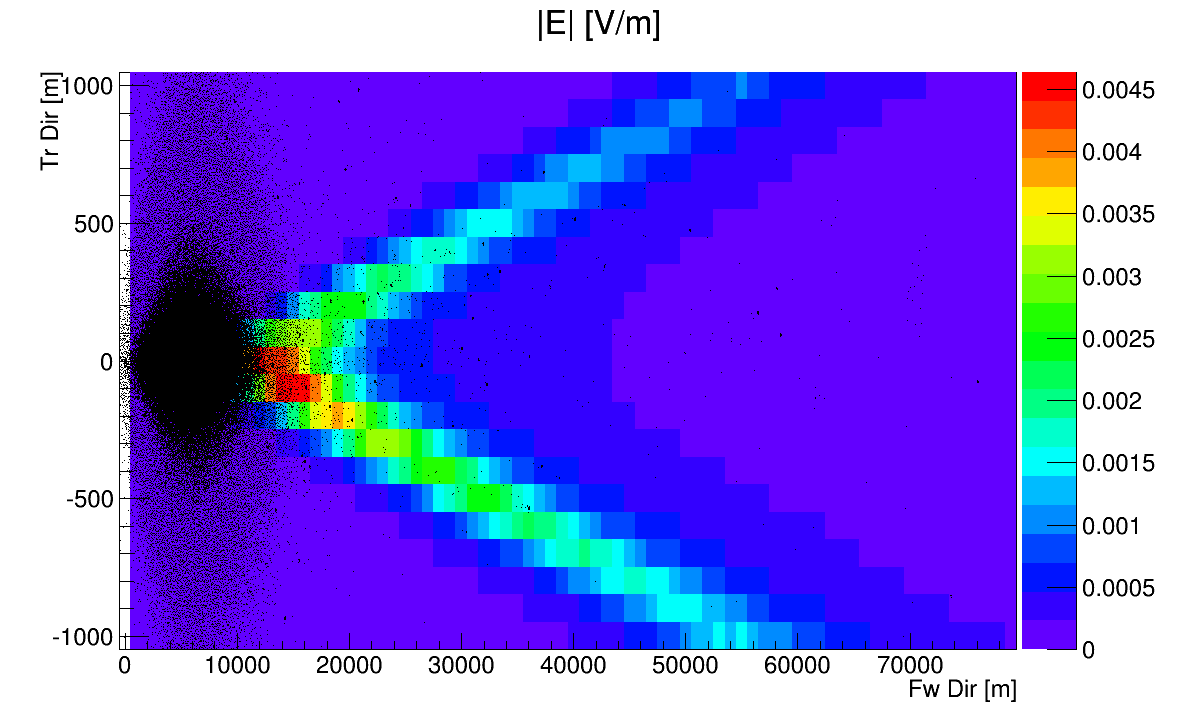
\includegraphics[width=\textwidth]{./fig/simulacionRadio/foorPrint_Test_18_89-5_90_25_1238_E_particles}
		\caption{\label{fig:sim_foot_y_part}
		Comparaci\'on entre la distribuci\'on de part\'iculas de la lluvia que alcanzan el suelo y la huella de campo el\'ectrico.
		}
	\end{figure}
	
	\subsection{Polarización de la señal - Influencia del campo magn\'etico terrestre}
	
	Otra car\'acter\'istica de la se\~nal que vale la pena estudiar es la polarizaci\'on del campo el\'ectrico en cada una de las antenas.
	Como primer paso, es posible utilizar los modelos macrosc\'opicos delineados en el cap\'itulo \ref{easRadio} para ganar intuici\'on al respecto. 
	Para ello, consideremos una lluvia completamente horizontal ($\theta=90^\circ$) que se desplaza de Oeste a Este ($\phi=90^\circ$) a alguna altura respecto del suelo.
	Bajo estas condiciones, y suponiendo que el campo magn\'etico terrestre es el de Tunka, es posible determinar la polarizaci\'on de la se\~nal en diferentes regiones del suelo.
	Para ello, basta con superponer en cada regi\'on las componentes geomagn\'eticas y Askaryan del campo generado, como se muestra en la figura \ref{fig:malField}.
	%
	\begin{figure}[ht!]
		\centering
		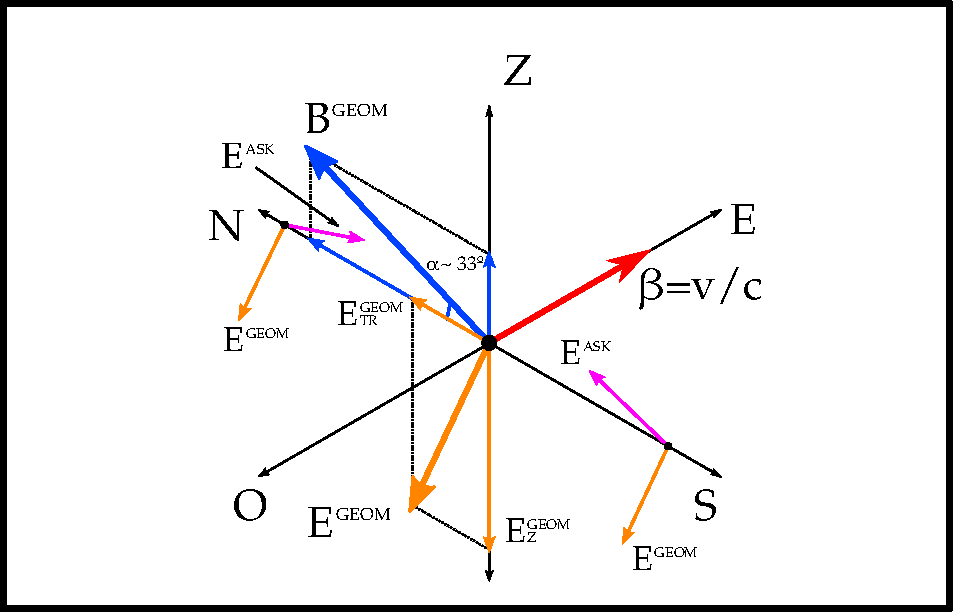
\includegraphics[width=0.8\textwidth]{./fig/simulacionRadio/malField}
		\caption{\label{fig:malField}
		Esquema de las componentes del campo elctrico para una lluvia que se desplaza de Oeste a Este en Tunka. Se considerarán los campos en el sistema de referencia definido por la lluvia, esto es, hacia arriba (componente $z$), y en las direcciones transversal (${\rm TR}$) y paralala (${\rm FW}$) a la dirección de propagación de la lluvia.
		El campo total es la suma de la contribución geomagnética, que conserva su dirección (transversal y hacia arriba) en todo el suelo y del aporte del efecto Askaryan, que tiene componentes transversales opuestas en el sector norte y el sur de la lluvia, mientras que su componente $z$ siempre es positiva.
		}
	\end{figure}
	%
	Por simplicidad es conveniente pensar en el campo en el sistema de referencia definido por la coordenada $z$ y las direcciónes paralela (${\rm FW}$) y transversal (${\rm TR}$) a la dirección de propagación sobre el suelo.
	Desde esta persectiva, a primer orden la contribución geomagnética al campo eléctrico tiene dirección $({\rm TR},z)$, ya que por construcción es perpendicular a la dirección de propagación.
	Por otro lado, a cada lado del eje de la lluvia la componente Askaryan tiene direcciones opuestas pero sobre el suelo siempre posee componente en $z>0$.
	
	Con esto en mente es posible estudiar la huella dejada por el evento de referencia, que posee caracter\'isticas muy similares al del ejemplo que se acaba de exponer~\footnote{Sus par\'ametros son los de la tabla \ref{tab:paramTestShower}.}.
	En las figuras \ref{fig:testFootprint_E0tr} y \ref{fig:testFootprint_E0z} se grafican el campo en dirección ${\rm TR}$ y en dirección $z$ de su huella.
	%
	\begin{figure}[ht!]
		\centering
		\includegraphics[width=\textwidth]{./fig/simulacionRadio/{foorPrint_ZWv1.22_ntuples_v1.21_ChTest_phi_90_18_89.5_90_25_1238_E0x_u}.png}
		\caption{\label{fig:testFootprint_E0tr}
		Huella de campo eléctrico en la dirección ${\rm TR}$. La intensidad del cono \cher{} es distinta a ambos lados del eje de la lluvia.
		Cuando la coordenada transversal es positiva el efecto Askaryan y el geomagnético se suprimen mientras que cuando es negativa se favorecen.
		}
	\end{figure}
	%
	Como puede observarse en \ref{fig:testFootprint_E0tr}, la intensidad del cono \cher{} en direcci\'on ${\rm TR}$ no es simétrica respecto del eje de la lluvia.
	Esto es consistente con lo que se esquematizó en la figura \ref{fig:malField}, que muestra que en la parte norte de la huella las contribuciones Askaryan y geomagnética en dirección ${\rm TR}$ se suprimen mientras que en la parte sur se favorecen.

	%
	\begin{figure}[ht!]
		\centering
		\includegraphics[width=\textwidth]{./fig/simulacionRadio/{foorPrint_ZWv1.22_ntuples_v1.21_ChTest_phi_90_18_89.5_90_25_1238_E0z_u}.png}
		\caption{\label{fig:testFootprint_E0z}
		Huella de campo eléctrico en la dirección $z$. En esta dirección las contribuciones geomagnética y Askaryan se suman en cualquier punto del suelo.
		}
	\end{figure}
	%
	Por otro lado, en \ref{fig:testFootprint_E0z} la componente $z$ del campo muestra una huella mucho más simétrica respecto del eje generado por la direcci\'on de propagaci\'on, consistente con que ambas contribuciones (geoagn\'etica y Askaryan) predicen una componente $z>0$ en toda la superficie.
	
	Por \'ultimo, en el ejemplo se despreció la componente ${\rm FW}$ del campo el\'ectrico.
	Dado que las lluvias ES son casi horizontales la aparición de esta componente a nivel del suelo se ve s\'umamente desfavorecida, como se observa en la figura \ref{fig:testFootprint_E0fw}.
	%
	\begin{figure}[ht!]
		\centering
		\includegraphics[width=\textwidth]{./fig/simulacionRadio/{foorPrint_ZWv1.22_ntuples_v1.21_ChTest_phi_90_18_89.5_90_25_1238_E0y_u}.png}
		\caption{\label{fig:testFootprint_E0fw}
		Campo eléctrico en la dirección ${\rm FW}$. Su intensidad es dos \'ordenes de magnitud menor que en las direcciones ${\rm TR}$ y $z$.
		}
	\end{figure}
	%
	Si se compara su intensidad con la de las huellas de las figuras \ref{fig:testFootprint_E0tr} y \ref{fig:testFootprint_E0z}, \'esta es dos \'ordenes de magnitud menor.
	Si bien en el ejemplo simplificado de la figura \ref{fig:malField} esta componente es nula, la leve inclinacion del evento de referencia ($\theta=90.5^\circ$) y posiblemente efectos de segundo \'orden generan su aparici\'on.
	
	\subsubsection{Polarizaci\'on del campo como filtro de antenas esp\'ureas}

	La regularidad que presenta la polarizaci\'on a lo largo de la huella puede ser explotada para eliminar de los eventos antenas con se\~nal esp\'urea.
	En la figura \ref{fig:footprintPolariz} se muestra la distribuci\'on de \'angulo azimutal ($0^\circ$ hacia el norte) y cenital del campo para las antenas cuya se\~nal supera los \cant{50}{\mu V/m}.
	%
	\begin{figure}[ht!]
		\centering
		\includegraphics[width=\textwidth]{./fig/simulacionRadio/{phiDist2DColz_Test_18_89.5_90_25_1238}.png}
		\includegraphics[width=\textwidth]{./fig/simulacionRadio/{thDist2DColz_Test_18_89.5_90_25_1238}.png}
		\caption{\label{fig:footprintPolariz}
		Distribuci\'on de \'angulo azimutal y cenital del campo el\'ectrico a lo largo de la huella de la lluvia. Se observa que el \'angulo azimutal se mantiene en valores \emph{cercanos} a cero mientras que el cenital no presenta var\'ia entre $0^\circ$ y $90^\circ$.
		}
	\end{figure}
	%
	Se observa que el \'angulo azimutal se mantienen en valores cercanos a cero mientras que el cenital var\'ia entre $0^\circ$ y $90^\circ$. 
	Entonces, si se quieren descartar antenas disparadas al azar resulta natural imponer una restricci\'on sobre el \'angulo azimutal del campo de cada antena de un evento. 
	Para definir esta restricci\'on es resulta \'util la figura \ref{fig:phiDist}, que muestra la distribuci\'on de $\phi$ en forma de histograma. 
	%
	\begin{figure}[ht!]
		\centering
		\includegraphics[width=\textwidth]{./fig/simulacionRadio/{phiDist_Test_18_89.5_90_25_1238}.png}
		\caption{\label{fig:phiDist}
		Histograma del \'angulo azimutal del evento. Se distinguen las entradas procedentes de la zona norte (sur) de la huella en las que se observan valores levemente sesgados negativamente (positivamente). Se observa que la mayor\'ia de las antenas presentan valores entre $-2.5^\circ$ y $2.5^\circ$, lo que da una idea del \'orden de magnitud del rango angular a seleccionar.
		}
	\end{figure}
	%
	
	Si bien se observa que en la zona norte y sur de la huella presentan valores en promedio distintos, el valor absoluto se mantiene por debajo de $2.5^\circ$ en la mayor\'ia de los casos, lo que define una zona de aceptaci\'on de alrededor de $\sim5^\circ$.
	Este valor permite entonces obtener una idea del orden de la reducci\'on en el numero de antenas con se\~nal al azar. 
	Bajo la hip\'otesis de que la polarizaci\'on del ruido es completamente aleatoria, la probabilidad de que una se\~nal esp\'urea aparezca en el rango definido por un evento sera $\sim 5/360\sim 1/60$.
	En resumen, un corte de selecci\'on en el \'angulo azimutal permitir\'ia rechazar alrededor del $98.5\%$ de las antenas disparadas por azar.
	Como consecuenta esta ganancia permitir\'ia bajar el nivel de disparo local de las antenas, aumentando la eficiencia a baja energ\'ia (ver secci\'on \ref{sbsc:depEvRadio}).
	
% 	\textbf{XXX ACA PODRIA AGREGAR lo de Bon y Boff y alguna evolucion del espectro o el espectro mismo}
	
	
	
% 	\begin{figure}[ht!]
% 		\centering
% 		\includegraphics[width=\textwidth]{./fig/simulacionRadio/{foorPrint_ZWv1.22_ntuples_v1.22_ChTest_phi_90_18_89.5_90_25_1238_E}.png}
% 		\includegraphics[width=\textwidth]{./fig/simulacionRadio/{foorPrint_ZWv1.22_ntuples_v1.22_ChTest_phi_90_18_89.5_90_25_1238_E0}.png}
% 		\caption{\label{fig:footprint_E_HEnv}
% 		asd
% 		}
% 	\end{figure}
% 	
% 	\begin{figure}[ht!]
% 		\centering
% 		\includegraphics[width=\textwidth]{./fig/simulacionRadio/{foorPrint_ZWv1.22_ntuples_v1.22_ChTest_phi_90_18_89.5_90_25_1238_EHB}.png}
% 		\includegraphics[width=\textwidth]{./fig/simulacionRadio/{foorPrint_ZWv1.22_ntuples_v1.22_ChTest_phi_90_18_89.5_90_25_1238_ELB}.png}
% 		\caption{\label{fig:footprint_HB-LB_HEnv}
% 		asd
% 		}
% 	\end{figure}
% 	
% 	\begin{figure}[ht!]
% 		\centering
% 		\includegraphics[width=\textwidth]{./fig/simulacionRadio/{foorPrint_ZWv1.22_ntuples_v1.22_ChTest_phi_90_18_89.5_90_25_1238_E}.png}
% 		\includegraphics[width=\textwidth]{./fig/simulacionRadio/{foorPrint_ZWv1.22_ntuples_v1.22_ChTest_phi_90_18_89.5_90_25_1238_E0}.png}
% 		\caption{\label{fig:footprint_E_HEnv}
% 		asd
% 		}
% 	\end{figure}
% 	
% 	\clearpage
	
	
	
% 	\begin{figure}[ht!]
% 		\centering
% 		\includegraphics[width=\textwidth]{./fig/simulacionRadio/{ZHSEvent_18_89.5_0_25_On_1238_E}.png}
% 		\includegraphics[width=\textwidth]{./fig/simulacionRadio/{ZHSEvent_18_89.5_0_25_Off_1238_E}.png}
% 		\caption{\label{fig:testFootprint_Ez}
% 		asd
% 		}
% 	\end{figure}
% 	
% 	\begin{figure}[ht!]
% 		\centering
% 		\includegraphics[width=\textwidth]{./fig/simulacionRadio/{ZHSEvent_18_89.5_0_25_On_1238_Ey}.png}
% 		\includegraphics[width=\textwidth]{./fig/simulacionRadio/{ZHSEvent_18_89.5_0_25_Off_1238_Ey}.png}
% 		\caption{\label{fig:testFootprint_Ez}
% 		asd
% 		}
% 	\end{figure}
% 	
% 	\begin{figure}[ht!]
% 		\centering
% 		\includegraphics[width=\textwidth]{./fig/simulacionRadio/{ZHSEvent_18_89.5_0_25_On_1238_Ez}.png}
% 		\includegraphics[width=\textwidth]{./fig/simulacionRadio/{ZHSEvent_18_89.5_0_25_Off_1238_Ez}.png}
% 		\caption{\label{fig:testFootprint_Ez}
% 		asd
% 		}
% 	\end{figure}
% 	
% 		\begin{figure}[ht!]
% 		\centering
% 		\includegraphics[width=\textwidth]{./fig/simulacionRadio/{ZHSEvent_18_89.5_0_25_On_1238_Ex}.png}
% 		\includegraphics[width=\textwidth]{./fig/simulacionRadio/{ZHSEvent_18_89.5_0_25_Off_1238_Ex}.png}
% 		\caption{\label{fig:testFootprint_Ez}
% 		asd
% 		}
% 	\end{figure}
% 	
% 	Bon y Boff
% 	
% 	mostrar que los efectos son comparables.
% 	
% 	velocidad de drift peque\~na por alra densidad en la atmósfera.
	
	
% 	\subsection{Evoluci\'on de la se\~nal a nivel del suelo}
% 		
% 	
% 	mostrar evolucion del EMax a lo largo de la lluvia
% 	
% 	mostrar espectro y evolucion
% 	
% 	mostrar fit del maximo de la lluvia como funcion de xd y theta y dependencia con la energia
% 	
% 		\subsubsection{Evoluci\'on de la polarizaci\'on}
% 		
% 		cambio askaryan geomagnetico?
% 	\clearpage
	
% 	\subsection{Caracterizaci\'on temporal}
% 	
% 	Velocidad de propagacion de la se\~nal.
% 	
	\section{Dependencia en los par\'ametros la lluvia}
	
	A fin de cuentas la exposici\'on a neutrinos depende de dos factores, las probabilidades de que se de inicio a una lluvia de par\'ametros $\Gamma$ y la eficiencia con la que estas son detectadas.
	Mientras que en este tipo de experimentos la modificaci\'on de las probabilidades de interacci\'on suele ser una tarea fuera del alcance\footnote{Estas dependen b\'asicamente del blanco con el que interact\'uan los neutrinos, que para detectores de superficie que observan eventos ES es la corteza de La Tierra. Un cambio en estas probabilidades implicar\'ia cambiar la locaci\'on del detector.}, las eficiencias de detecci\'on pueden ser controladas con cierta libertad variando el dise\~no del detector. 
	Por este motivo resulta clave entender c\'omo cambia la huella de radio de los eventos ES al variar los distintos par\'ametros de la lluvia que la genera.
	As\'i, a partir de este conocimiento y del estudio de las probabilidades de interacci\'on ser\'a posible por un lado optimizar el dise\~no del detector y por otro definir el espacio de par\'ametros sobre el que es necesario simular eventos.
	
	En la secci\'on \ref{sbsc:localTriggerRadio} se decidi\'o que la condici\'on de disparo de cada antena dependa de del campo el\'ectrico m\'aximo registrado sobre la misma.
	Por este motivo el \'area sobre la cu\'al la huella de la radio supera el umbral de detecci\'on resulta ser una variable altamente relacionada con el disparo global de los eventos.
	En la misma l\'inea el campo el\'ectrico m\'aximo registrado a lo largo de la huella permite inferir si un la lluvia tiene o no la capacidad de producir disparos locales.
	Por \'ultimo, como se discutir\'a en la secci\'on \ref{sc:identificacionRadio}, medidas del ancho de la huella se encuentran relacionadas con la posibilidad de distinguir eventos ES de las lluvias de fondo.
	Con todo esto en mente, en las siguientes secciones se estudiar\'a el comportamiento de algunas de estas variables al cambiar los par\'ametros del evento de referencia.
	
	\subsection{Efecto del \'angulo cenital $\theta$}
	\label{sbsc:depThetaRadio}
	
% 	En primer lugar se estudiar\'a c\'omo cambia la huella al variar el \'angulo cenital del evento.
	Debido a la geometr\'ia del cono \cher{} existir\'a un \'angulo m\'aximo a partir del cu\'al la emisi\'on de radio de la lluvia no interactuar\'a con el detector~\footnote{Esto significa que la compresi\'on temporal no ser\'a suficiente para imprimir una se\~nal apreciable en las antenas.}.
	Seg\'un el modelo simplificado presentado en la secci\'on \ref{sc:toymodelES} \'este \'angulo de corte deber\'ia ser cercano a $1.4^\circ$, como lo indica la figura \ref{fig:chConeWidth}.
	
	\begin{figure}[ht!]
		\centering
		\begin{tabular}{cc}
		$90.1^\circ$ & $90.5^\circ$ \\
		\includegraphics[width=0.5\textwidth]{./fig/simulacionRadio/theta/{foorPrint_ZWv1.21_ntuples_v1.21_Misc_phi_90_18_89.9_90_25_1238_E0}.png} &
		\includegraphics[width=0.5\textwidth]{./fig/simulacionRadio/theta/{foorPrint_ZWv1.21_ntuples_v1.21_Misc_phi_90_18_89.5_90_25_1238_E0}.png}\\
		
		$90.9^\circ$ & $91.3^\circ$ \\
		\includegraphics[width=0.5\textwidth]{./fig/simulacionRadio/theta/{foorPrint_ZWv1.21_ntuples_v1.21_Misc_phi_90_18_89.1_90_25_1238_E0}.png} &
		\includegraphics[width=0.5\textwidth]{./fig/simulacionRadio/theta/{foorPrint_ZWv1.21_ntuples_v1.21_Misc_phi_90_18_88.7_90_25_1238_E0}.png}\\
		
		$91.7^\circ$ & $92.3^\circ$ \\
		\includegraphics[width=0.5\textwidth]{./fig/simulacionRadio/theta/{foorPrint_ZWv1.21_ntuples_v1.21_Misc_phi_90_18_88.3_90_25_1238_E0}.png} &
		\includegraphics[width=0.5\textwidth]{./fig/simulacionRadio/theta/{foorPrint_ZWv1.21_ntuples_v1.21_Misc_phi_90_18_87.7_90_25_1238_E0}.png}\\
		\end{tabular}
		\caption{\label{fig:theta_dependence}
		Huella sobre el detector del evento de referencia, para diferentes \'angulos cenitales. En todos los casos la lluvia se inici\'o en $(x,y)=(0,0)$. Se observa como al aumentar el \'angulo cenital el punto de impacto del cono \cher{}
		(que se encuentra determinado aproximadamente por la antena con m\'axima se\~nal)
		se aleja del punto de inicio de la lluvia, en acuerdo con la figura \ref{fig:chConeWidth} del cap\'itulo \ref{ch:easRadio}. Por otro lado, es posible notar como el m\'aximo de la huella disminuye dos \'ordenes de magnitud al variar cerca de $2.5^\circ$ de \'angulo cenital.
		}
	\end{figure}
	
	Para estudiar la situaci\'on la figura \ref{fig:theta_dependence} muestra la huella dejada sobre el detector por el evento de referencia con distintos \'angulos ceintales.
	Dado que en todos los casos el \tauon{} decay\'o en $(x,y)=(0,0)$, el punto de impacto del cono \cher{} se desplaza hacia valores positivos de $x$ a medida que $\theta$ crece.
	Sumado a este efecto, la amplitud de la huella en general disminuye, lo que puede deberse tanto al factor $1/R$ como a un efecto de compresi\'on de la se\~nal.
	A fin de cuentas este hecho sugiere que existir\'a un \'angulo m\'aximo a partir del cu\'al los eventos ES no poseen la capacidad de disparar el detector.
% 	En particular, para valores superiores a $\sim91.3^\circ$ el m\'aximo de se\~nal coherente no alcanza el detector, lo que genera un corte en la eficiencia de detecci\'on.
	
	Para apoyar este punto en la figura \ref{fig:theta_dependence2} se muestra el campo el\'ectrico m\'aximo de la lluvia para diferentes \'angulos cenitales y energ\'ias.
	%
	\begin{figure}[ht!]
		\centering
		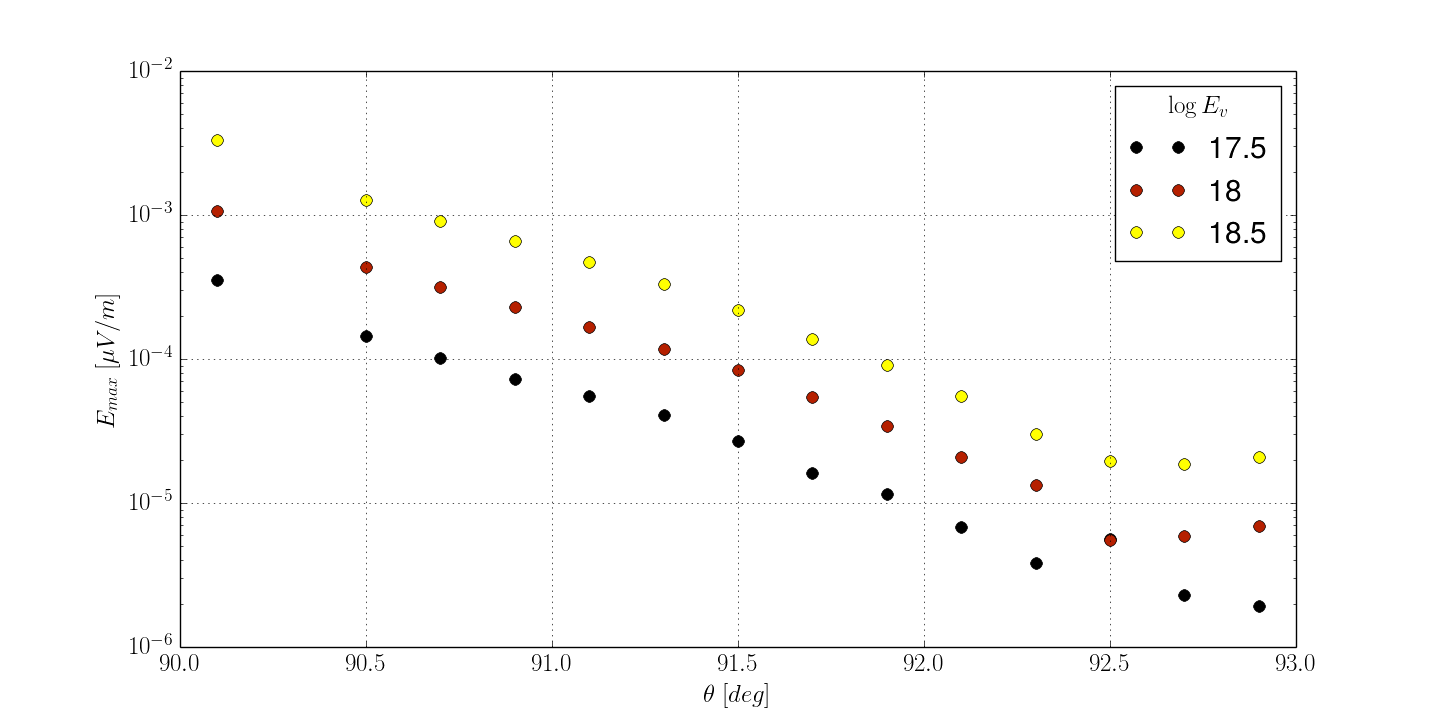
\includegraphics[width=\textwidth]{./fig/simulacionRadio/maxDep/eMaxTh}
		\caption{\label{fig:theta_dependence2}
		M\'aximo campo el\'ectrico de la lluvia como funci\'on del \'angulo cenital, para distintos valores de \ev{}. El decaimiento es aproximadamente exponencial.
		}
	\end{figure}
	%
	Dicha variable presenta un decaimiento aproximadamente exponencial hasta cerca de $92.5^\circ$ donde el comportamiento cambia.
	Para este \'angulo incluso a \cant{E_v=10^{18.5}}{eV} el m\'aximo de la huella no alcanza niveles detectables (\cant{\sim25}{\mu V/m}),
% 	, lo que .
% 	Este comportamiento tambien se observa para diferentes alturas de decaimiento del \tauon{}
	por lo que se lo considerar\'a como valor de corte y no se simular\'an eventos cuyo \'angulo cenital supere los $\sim92.5^\circ$.
	
	\subsection{Efecto de altura de decaimiento del tauon \xd{}}
	\label{sbsc:depXdRadio}
	
	Tambien resulta interesante estudiar como cambia la huella del campo el\'ectrico al variar la altura de decaimiento del \tauon{} en el evento de referencia, lo que se muestra en la figura \ref{fig:xd_dependence} para \cant{{\rm x_d} = \left\{25,75,150,300\right\}}{m}. 
	%
	\begin{figure}[ht!]
		\centering
		\begin{tabular}{cc}
		\cant{25}{m} & \cant{75}{m} \\
		\includegraphics[width=0.5\textwidth]{./fig/simulacionRadio/xd/{foorPrint_ZWv1.21_ntuples_v1.21_Misc_TestXd_18_89.5_90_25_1238_E0}.png} &
		\includegraphics[width=0.5\textwidth]{./fig/simulacionRadio/xd/{foorPrint_ZWv1.21_ntuples_v1.21_Misc_TestXd_18_89.5_90_75_1238_E0}.png}\\
		
		\cant{150}{m} & \cant{300}{m} \\
		\includegraphics[width=0.5\textwidth]{./fig/simulacionRadio/xd/{foorPrint_ZWv1.21_ntuples_v1.21_Misc_TestXd_18_89.5_90_150_1238_E0}.png} &
		\includegraphics[width=0.5\textwidth]{./fig/simulacionRadio/xd/{foorPrint_ZWv1.21_ntuples_v1.21_Misc_TestXd_18_89.5_90_300_1238_E0}.png}\\
		\end{tabular}
		\caption{\label{fig:xd_dependence}
		Huella sobre el detector del evento de referencia para distintas alturas de decaimiento. Se observa como a medida que aumenta la altura de decaimiento del \tauon{} la intensidad del campo el\'ectrico decrece.
		}
	\end{figure}
	%
	Una vez m\'as la huella se traslada hacia valores positivos de $x$ al aumentar el valor del par\'ametro \xd{}.
	Dado que la cascada se inici\'o en $(x,y)=(0,0)$ este corrimiento resulta compatible con el modelo del cono \cher{}~\footnote{Esto se entiende si se piensa que al variar \xd{} el plano del suelo corta el eje de la lluvia en diferentes posiciones, modificando el punto de impacto de la se\~nal.}.
	Cabe destacar que adem\'as de desplazarse, la intensidad de la huella disminuye a medida que aumenta \xd{}, lo que nuevamente puede deberse al decaimiento de $1/R$ del campo o a efectos de compresi\'on temporal de la se\~nal. 
	De manera an\'aloga a lo que ocure para el \'angulo cenital, esto sugiere la existencia de una altura de decaimiento a partir de la cual el campo sobre el detector no es suficiente para dispararlo.
	Entonces resulta \'util entonces estudiar c\'omo var\'ia el m\'aximo campo el\'ectrico de la huella para diferentes valores de altura de decaimiento y energ\'ia visible, lo que se muestra en la figura \ref{fig:xd_dependence2}.
	%
	\begin{figure}[ht!]
		\centering
		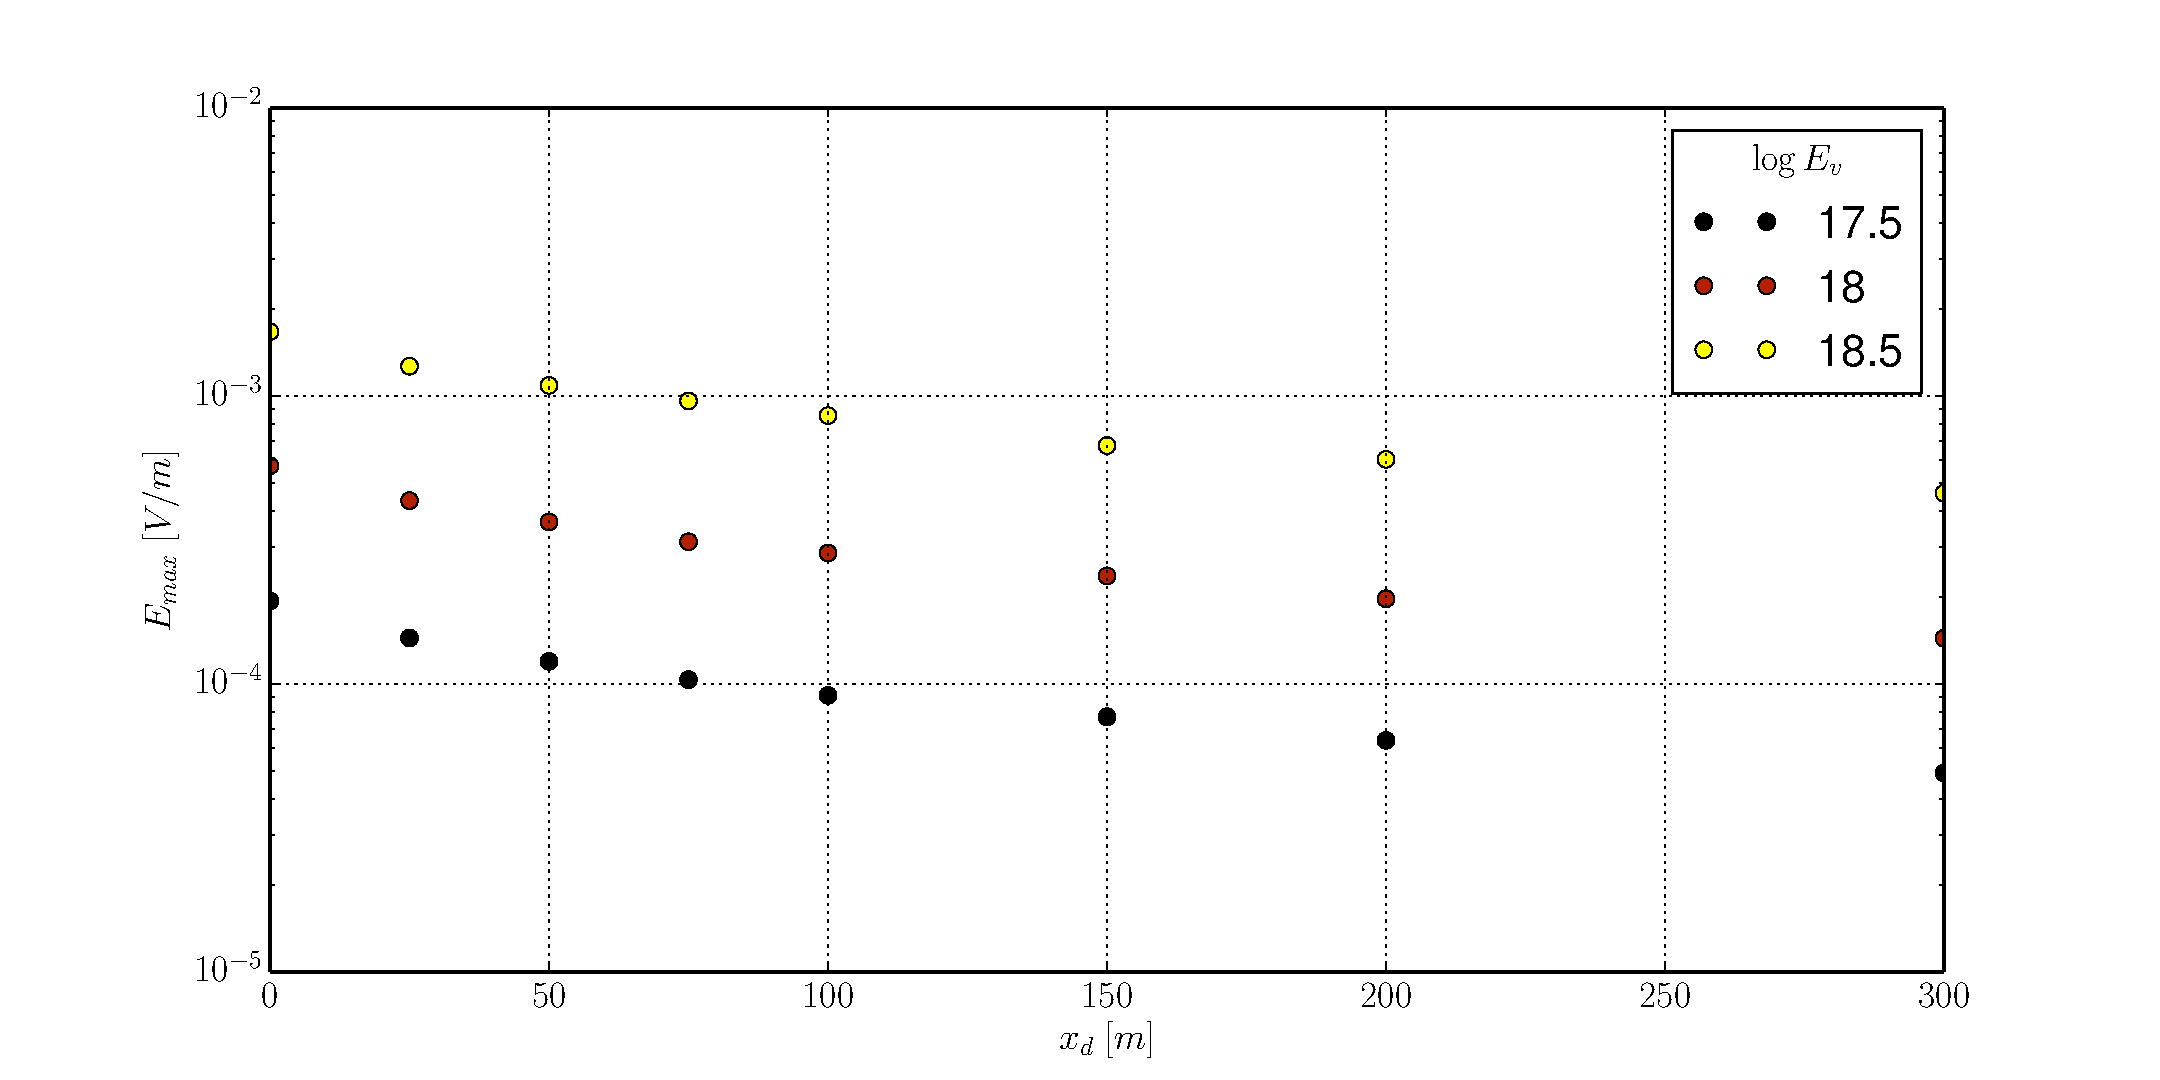
\includegraphics[width=\textwidth]{./fig/simulacionRadio/maxDep/eMaxXd}
		\caption{\label{fig:xd_dependence2}
		M\'aximo campo el\'ectrico de la lluvia como funci\'on de la altura de decaimiento del \tauon{}, para diferentes energ\'ias.
		Se observa un decaimiento aproximadamente exponencial.
		}
	\end{figure}
	
	Se observa como a medida que \xd{} aumenta esta variable decae, por lo que dado un valor de energ\'ia visible a partir de cierto valor de \xd{} ning\'un sector de la huella ser\'a capaz de dar trigger.
	A diferencia de lo que sucede con el \'angulo cenital, en el que el corte en $92.5^\circ$ es com\'un a todas las energ\'ias y alturas de decaimiento, el corte en \xd{} depende tanto de \ev{} como de $\theta$.
	Adem\'as, como se ver\'a mas adelante, este efecto tendr\'a importancia s\'olo a baja energ\'ia, mientras que para energ\'ias superioras a \cant{\sim10^{18}}{eV} la eficiencia a altos \xd{} se ver\'a suprimida por el efecto de la curvatura de la tierra (ver ap\'endice \ref{ap:tierraCurva} y cap\'itulo \ref{ch:resultadosRadio}).
	Por estos motivos, para cada bin de energ\'ia y \'angulo cenital se decidir\'a el m\'aximo \xd{} a simular basados en las posibilidades de disparar el detector.
	
	\subsection{Efecto del \'angulo azimutal $\phi$}
	\label{sbsc:depPhiRadio}
	En base a lo estudiado en el cap\'itulo \ref{ch:easRadio}, el efecto geomagn\'etico provoca que la distribuci\'on de campo el\'ectrico a nivel del suelo dependa del \'angulo azimutal.
	Para comprender mejor esta dependencia es interesante estudiar el t\'ermino $E(\phi)\propto\vec\beta(\phi)\times \vec B$ en Tunka\footnote{La declinaci\'on del campo geomagn\'etico en Tunka es de $71.2^\circ$.}.
	La figura \ref{fig:geomComps_Tunka} muestra la variaci\'on de las componentes $E_x$, $E_y$, $E_z$, $E_{TR}$ y $|E|$ con el \'angulo azimutal para un \'angulo cenital de $\theta=90.5^\circ$.
	%
	\begin{figure}[ht!]
		\centering
		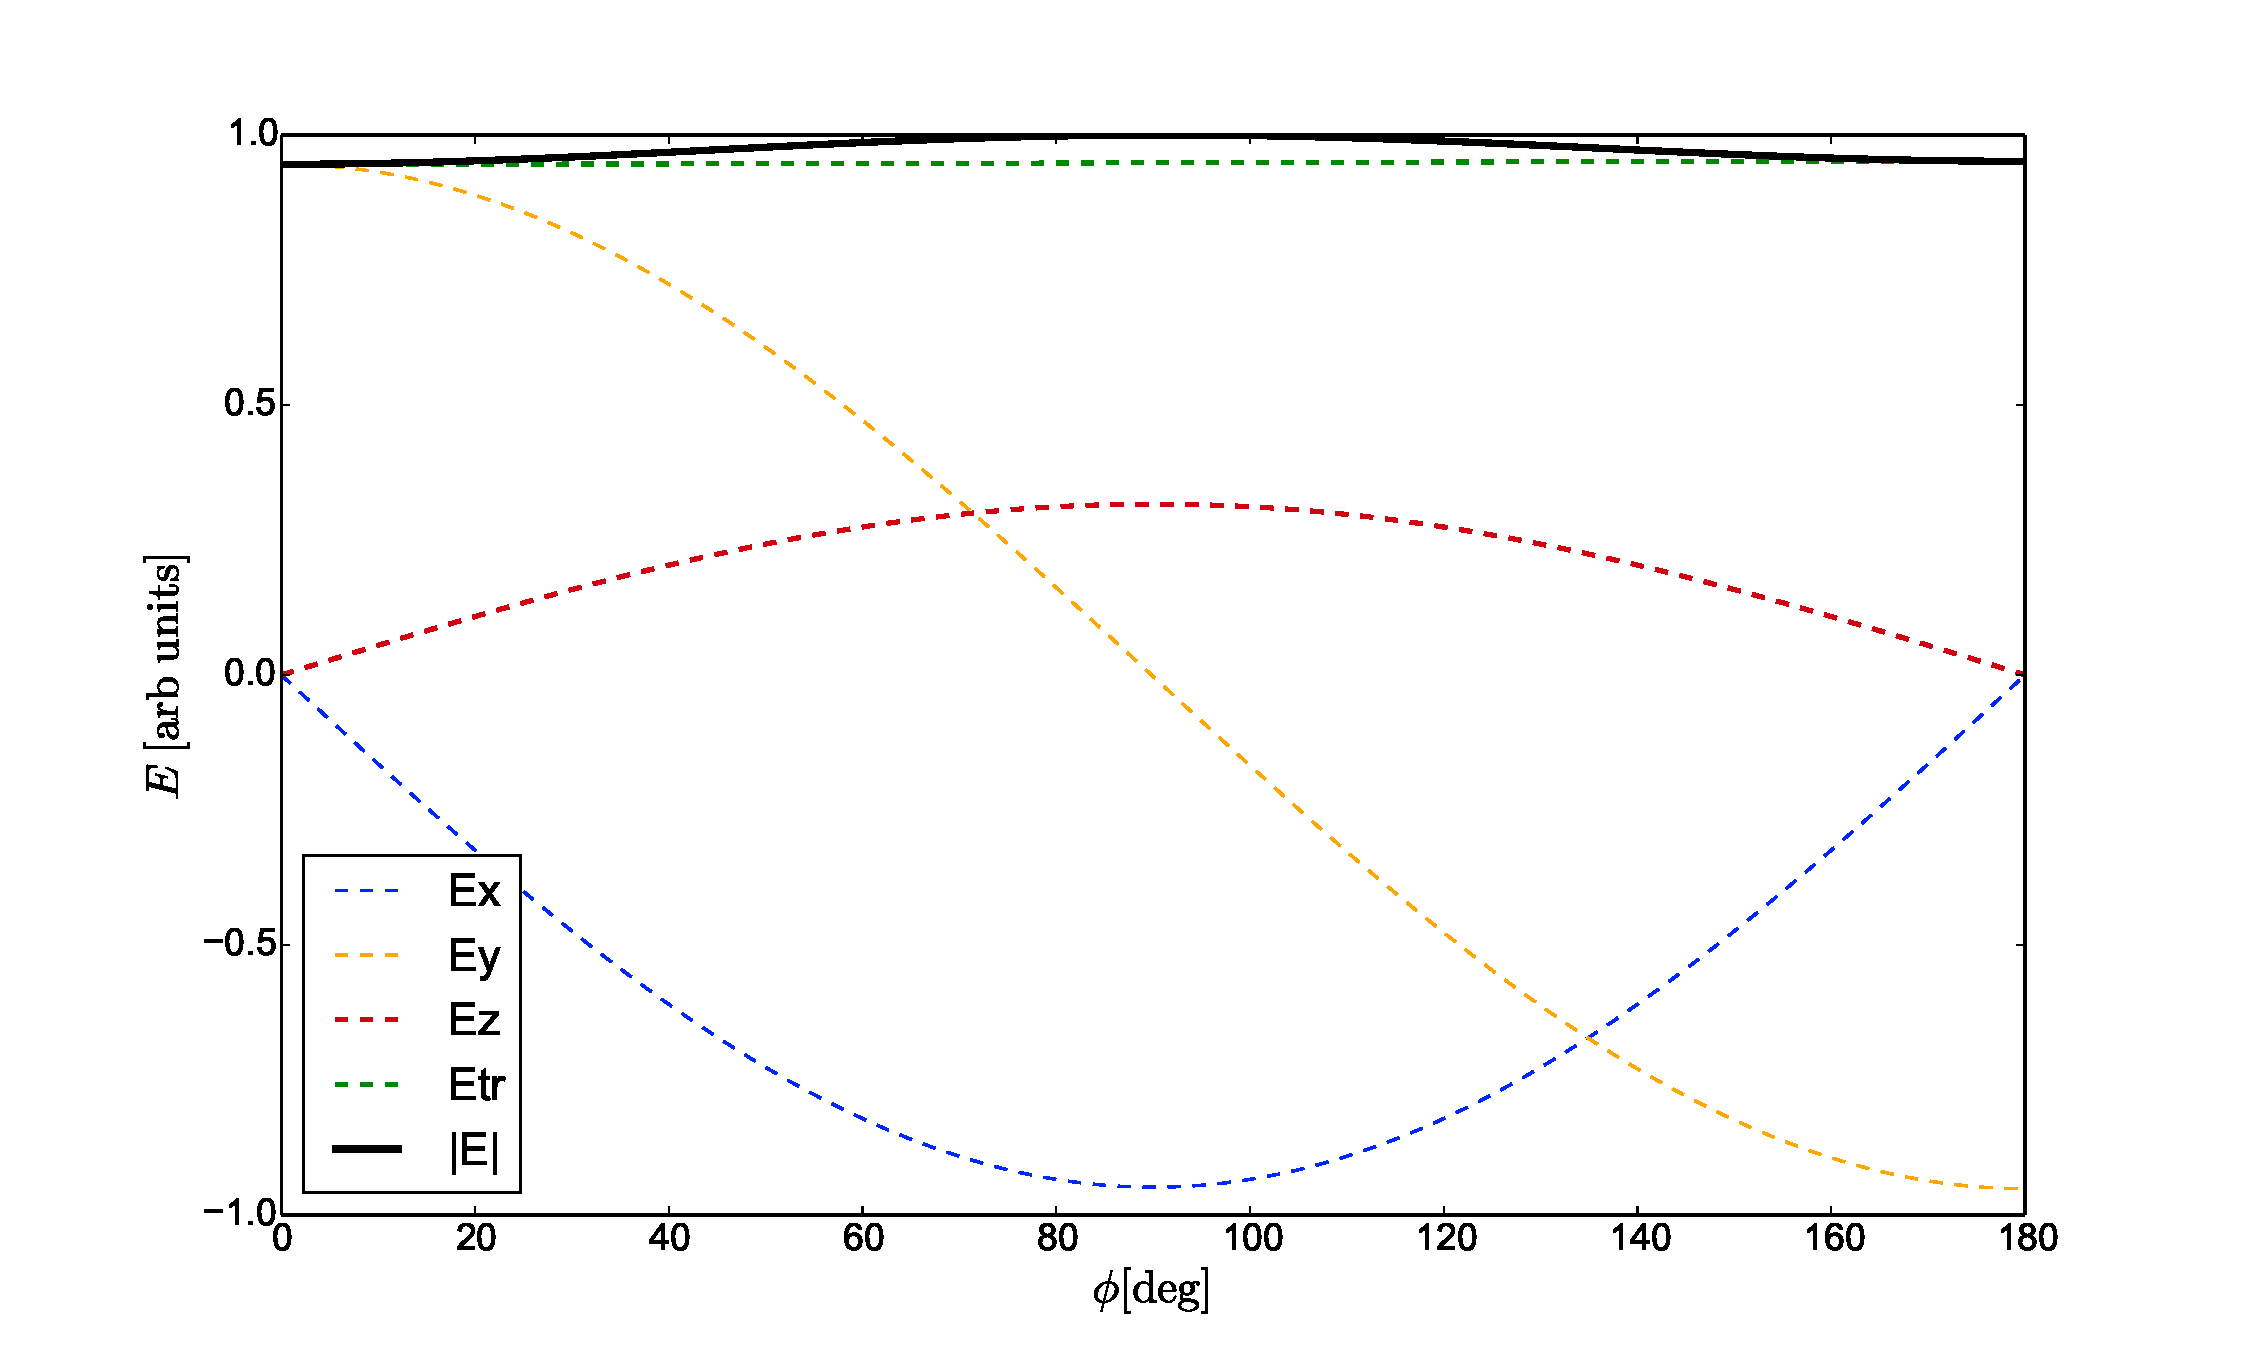
\includegraphics[width=\textwidth]{./fig/simulacionRadio/geomComps_Tunka}
		\caption{\label{fig:geomComps_Tunka}
		Componentes $E_x$, $E_y$, $E_z$, $E_{TR}$ y $|E|$ en funci\'on del \'angulo azimutal 
		$\phi$, calculados a partir de la ecuaci\'on $E(\phi)\propto\vec\beta(\phi)\times \vec B$. El campo geomagn\'etico utilizado tiene la declinaci\'on que se observa en Tunka,$71.2^\circ$. 
		}
	\end{figure}
	%
	Debido a que el campo geomagn\'etico en Tunka es casi vertical, si bien las componentes $E_x$ y $E_y$ var\'ian significativamente con $\phi$, la componente transversal $E_{TR}$ del campo se mantiene practicamente constante (l\'inea de trazos verde en \ref{fig:geomComps_Tunka}). 
	Esto se debe a que esta componente depende b\'asicamente de la proyecci\'on vertical del campo geomagn\'etico.
	La peque\~na variaci\'on que se aprecia aparece debido a que el c\'alculo se realiz\'o suponiendo una lluvia no horizontal.
	Por otro lado, debido a que $\vec B$ define el norte magn\'etico ($\phi=0^\circ$) la coponente $E_z$ vale 0 para $\phi=0^\circ$ y $\phi=180^\circ$ ($\vec\beta$, $\vec B$ y $\hat z$ son coplanares), y dado que su declinaci\'on es menor a $90^\circ$, esta componente tomar\'a un valor m\'aximo para $\phi=90^\circ$ (l\'inea de trazos roja en la figura). 
	Como resultado de estas dos constribuciones, el m\'odulo total del campo el\'ectrico $|E|$ muestra una variaci\'on de aproximadamente $10\%$ entre 0 y 180 grados. 
	
	Con esto en mente resulta interesante entonces observar como se modifica la huella de $|E|$ del evento de referencia al cambiar el \'angulo azimutal entre $\phi=0^\circ$ y $\phi=90^\circ$, lo que se muestra para el evento de referencia en la figura \ref{fig:phi_dependence}. 
	\begin{figure}[ht!]
		\centering
		\begin{tabular}{cc}
		$0^\circ$ & $90^\circ$ \\
		\includegraphics[width=0.5\textwidth]{./fig/simulacionRadio/phi/{foorPrint_ZWv1.21_ntuples_v1.21_Misc_TestPhi_18_89.5_0_25_1238_E0}.png} &
		\includegraphics[width=0.5\textwidth]{./fig/simulacionRadio/phi/{foorPrint_ZWv1.21_ntuples_v1.21_Misc_TestPhi_18_89.5_90_25_1238_E0}.png}\\
		
		\end{tabular}
		\caption{\label{fig:phi_dependence}
		Huella sobre el detector del evento de referencia para $\phi=0^\circ$ y $\phi=90^\circ$.
		}
	\end{figure}
	En acuerdo con la figura \ref{fig:geomComps_Tunka} la huella para $\phi=0^\circ$ en promedio valores de campo el\'ectrico menores que para $\phi=90^\circ$, sin embargo, la variaci\'on a lo largo de la huella resulta mayor a $10\%$.
	Esta diferencia puede deberse a que el cambio de direcci\'on de la contribuci\'on del efecto geomagn\'etico provoque una cancelaci\'on diferente con la contribuci\'on Askaryan en cada caso.
	
	\subsection{Efecto de la eneg\'ia visible $E_v$}
	\label{sbsc:depEvRadio}
	De acuerdo con lo expuesto en el cap\'itulo \ref{ch:easAuger} y en particular en la ecuaci\'on \ref{hi4}, el n\'umero de part\'iculas en el m\'aximo de la lluvia escala con la energ\'ia del primario o, el par\'ametro equivalente en eventos ES, la energ\'ia visible \ev{}.
	Por otra parte, dado que la emisi\'on de radio depende directamente del n\'umero de part\'iculas en el m\'aximo de la lluvia, resulta razonable suponer que la intensidad del campo el\'ectrico a nivel del suelo variar\'a tambien proporcionalmente a \ev{}.
	Para estudiar este efecto, en la figura \ref{fig:ev_dependence} se muestra la huela dejada por el evento de referencia con \cant{E_v=\left\{10^{17.5},10^{18},10^{18.5}\right\}}{eV}.
	Nuevamente el punto de inicio de la lluvia es $(x,y)=(0,0)$, y puede observarse como el campo el\'ectrico aumenta en intensidad a medida que aumenta la energ\'ia visible.
	%
	\begin{figure}[ht!]
		\centering
		\begin{tabular}{cc}
		\cant{10^{17.5}}{eV} & \cant{10^{18}}{eV}\\
		\includegraphics[width=0.5\textwidth]{./fig/simulacionRadio/ev/{foorPrint_ZWv1.21_ntuples_v1.21_Misc_TestEv_17.5_89.5_90_25_1238_E0}.png} &
		\includegraphics[width=0.5\textwidth]{./fig/simulacionRadio/ev/{foorPrint_ZWv1.21_ntuples_v1.21_Misc_TestEv_18_89.5_90_25_1238_E0}.png}\\
		
		\multicolumn{2}{c}{\cant{10^{18.5}}{eV}} \\
		\multicolumn{2}{c}{\includegraphics[width=0.5\textwidth]{./fig/simulacionRadio/ev/{foorPrint_ZWv1.21_ntuples_v1.21_Misc_TestEv_18.5_89.5_90_25_1238_E0}.png}}\\
		
		\end{tabular}
		\caption{\label{fig:ev_dependence}
		Huella sobre el detector del evento de referencia con \cant{E_v=\left\{10^{17.5},10^{18},10^{18.5}\right\}}{eV}.
		Se observa como a medida que aumenta \ev{} la intensidad del campo el\'ectrico aumenta.
		}
	\end{figure}
	
	Para reforzar la idea la figura \ref{fig:ev_dependence2} muestra como var\'ia el m\'aximo campo el\'ectrico de la lluvia con la energ\'ia para diversos valores de \'angulos cenitales y alturas de decaimiento.
	%
	\begin{figure}[ht!]
		\centering
		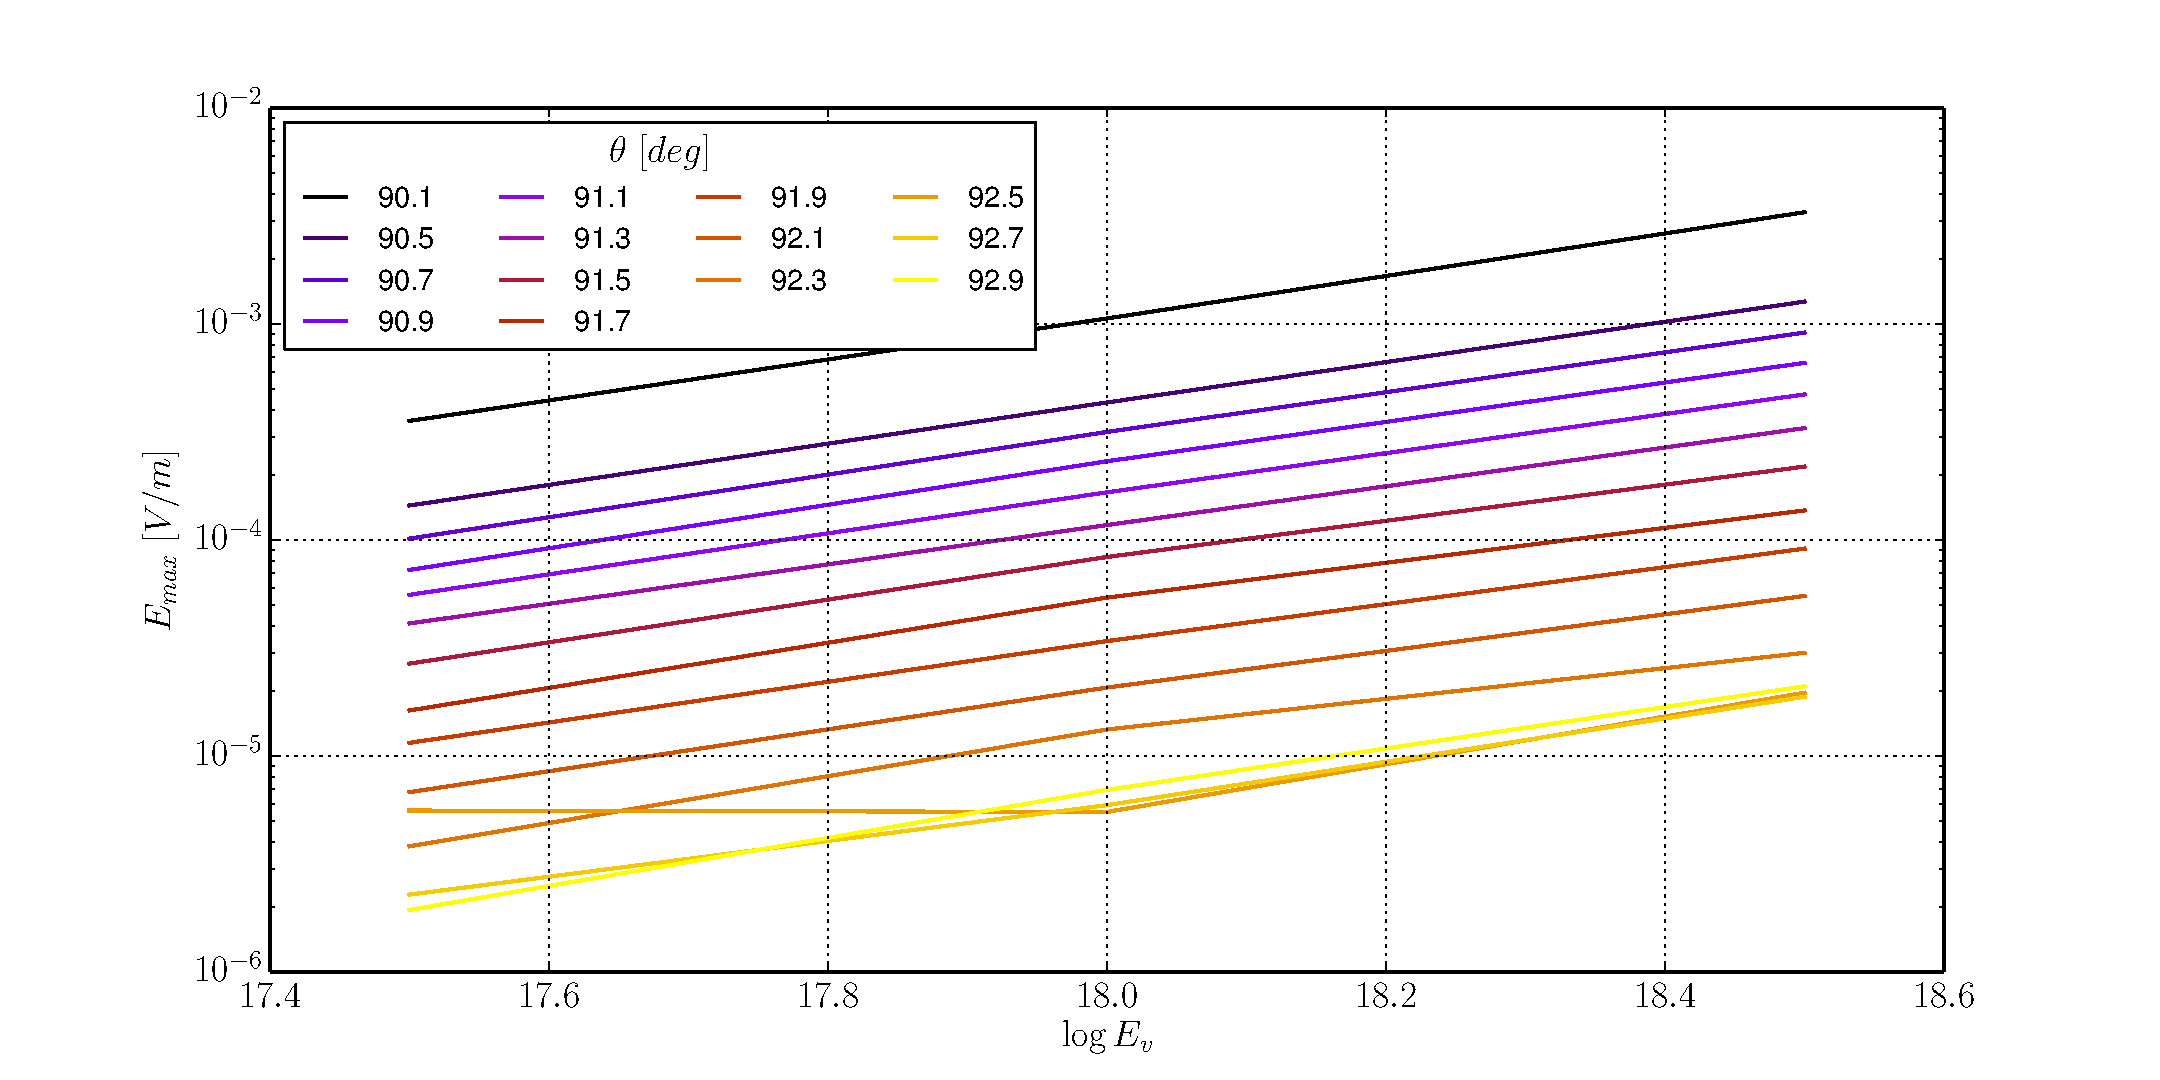
\includegraphics[width=\textwidth]{./fig/simulacionRadio/maxDep/eMaxThEv}
		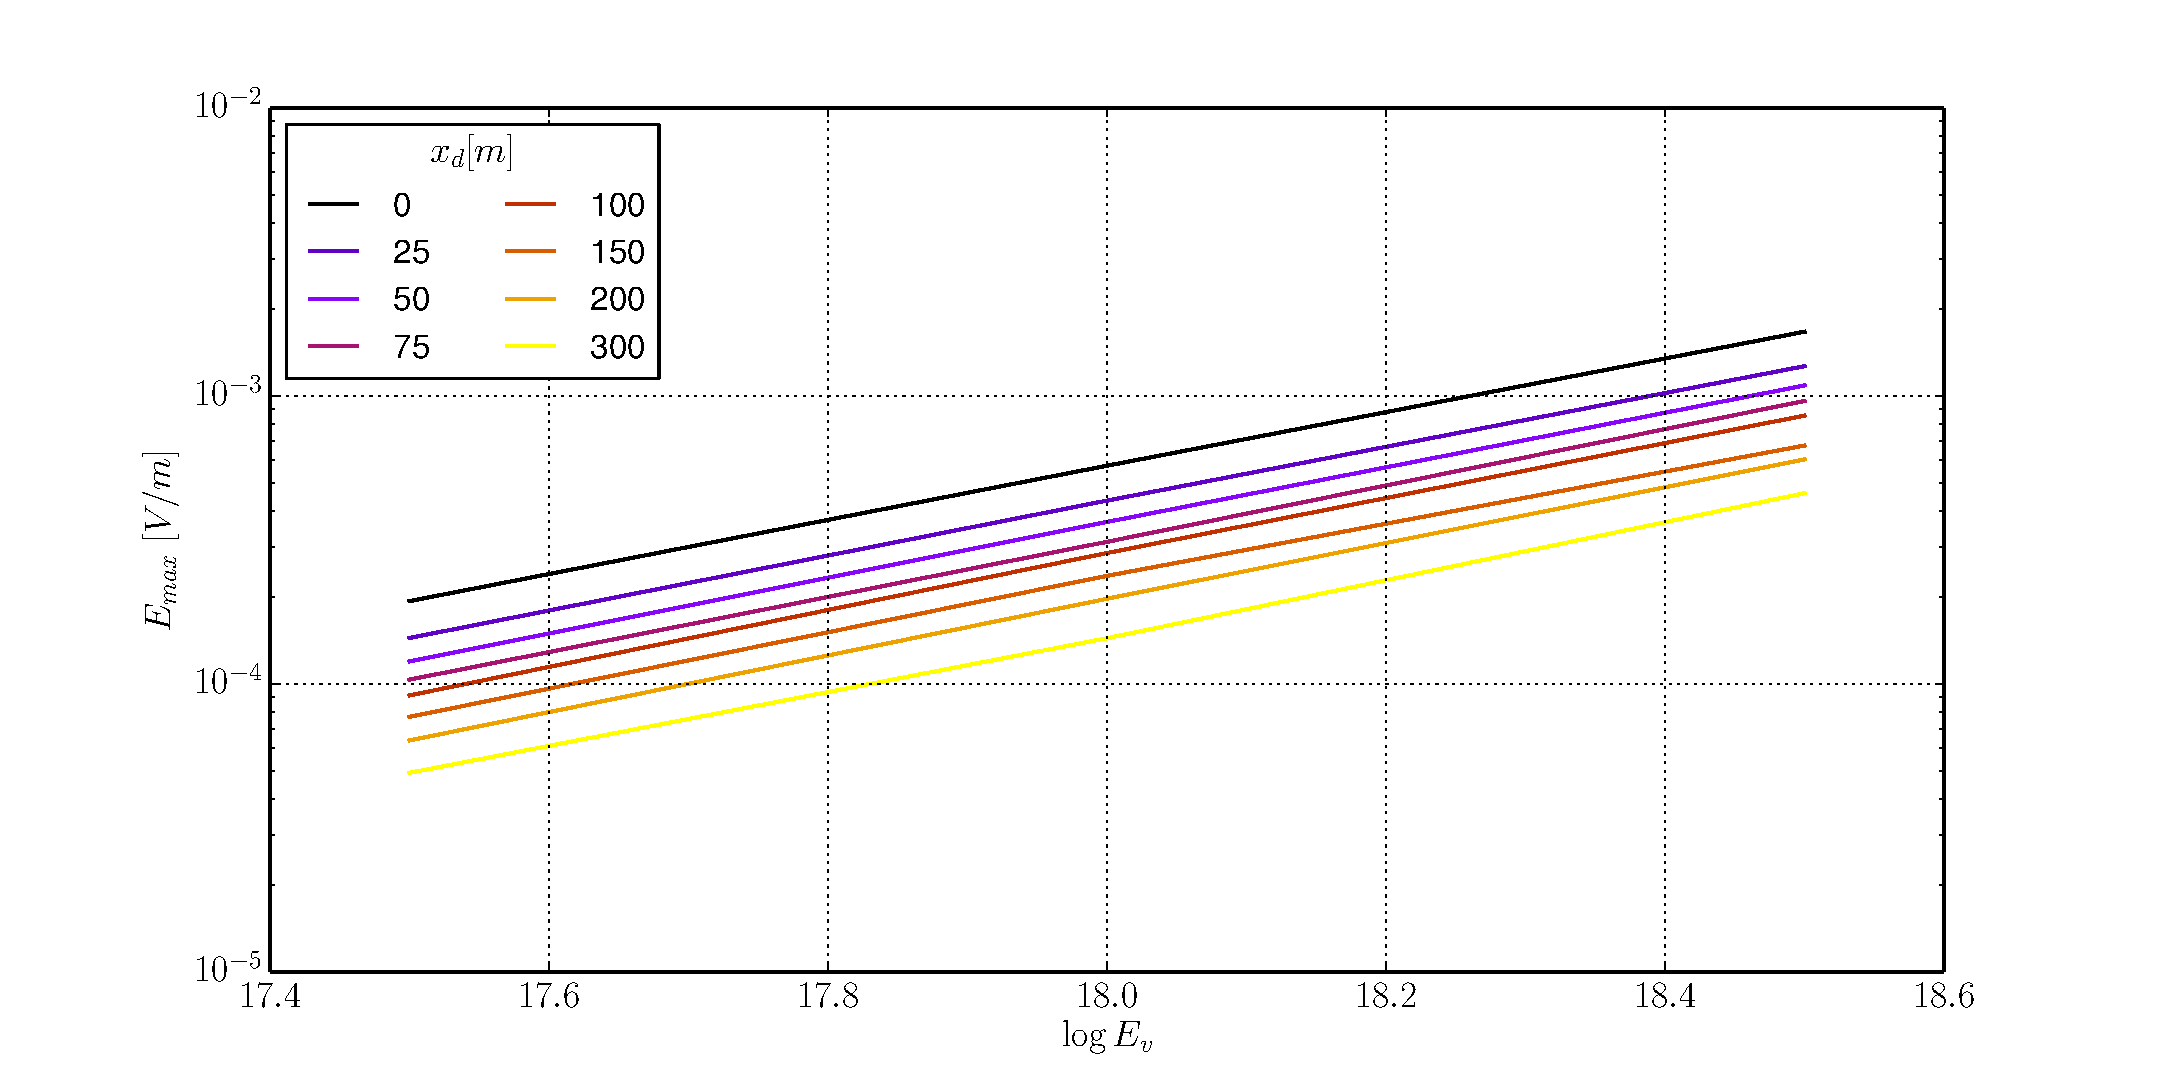
\includegraphics[width=\textwidth]{./fig/simulacionRadio/maxDep/eMaxXdEv}
		\caption{\label{fig:ev_dependence2}
		Arriba (Abajo): M\'aximo campo el\'ectrico registrado en la huella en funci\'on del logaritmo de la energ\'ia visible para varios \'angulos cenitales (varias alturas de decaimiento del \tauon{}).
		Esta cantidad resulta proporcional a la energ\'ia visible en todos los casos.
		}
	\end{figure}
	%
	En todos los casos la dependencia de con la energ\'ia es pr\'acticamente lineal.
	Este comportamiento creciente sugiere, que a medida que aumente la energ\'ia visible de la lluvia la eficiencia de detecci\'on crecer\'a.
	
	
	\subsection{Dependencia con el canal de decaimiento del \tauon{}}
	\label{sbsc:decayChRadio}
	
	Finalmente es necesario estudiar como afecta el canal de decaimiento del \tauon{} a la huella de radio sobre el detector.
	Dado que el par\'ametro de control de energ\'ia elegido en esta parte de la tesis es la energ\'ia visible, es decir, la que portan las part\'iculas poco penetrantes al inicio de la lluvia, el canal de decaimiento queda determinado por las part\'iculas la inician y por como se distribuye la energ\'ia entre ellas\footnote{Como contraparte, en el an\'alisis para Auger lo que determinaba el decaimiento del \tauon{}, ademas de las part\'iculas y la distribuci\'on de energ\'ia, es qu\'e fracci\'on de la energ\'ia del tau\'on se transmitia a las part\'iculas interactuantes.}.
	Por otro lado, ya se ha expuesto que la emisi\'on de radio en lluvias atmosf\'ericas extendidas depende fuertemente de el n\'umero de part\'iculas que se generan durante su evoluci\'on que a su vez, dada la universalidad de las EAS, se encuentra estrechamente relacionado con la energ\'ia del primario.
	Entonces, a la luz de estos dos hechos se espera que a misma energ\'ia visible y par\'ametros geom\'etricos, el canal de decaimiento del \tauon{} no afecte las caracter\'isticas fundamentales de la huella de radio sobre el detector.
	Para poner a prueba esta hip\'otesis, en la figura \ref{fig:tdec_dependence} se muestra la se\~nal a nivel del suelo para cuatro de los canales de decaimiento m\'as representativos. Se observa que las caracter\'isticas generales de la huella se conserva en todos los casos, aunque var\'ia levemente en forma e intensidad.
	%
	\begin{figure}[ht!]
		\centering
		\begin{tabular}{cc}
		$\tau\rightarrow\nu_\tau\pi^-$ - BR=10.9$\%$ & $\tau\rightarrow\nu_\tau\pi^-\pi^-\pi^+$ - BR=9.3$\%$ \\
		\includegraphics[width=0.5\textwidth]{./fig/simulacionRadio/decay/{foorPrint_Cone_ZWv1.22_ntuples_v1.21_ChTest_phi_90_18_89.5_90_25_1005_E0_u}.png} &
		\includegraphics[width=0.5\textwidth]{./fig/simulacionRadio/decay/{foorPrint_Cone_ZWv1.22_ntuples_v1.21_ChTest_phi_90_18_89.5_90_25_1023_E0_u}.png}\\
		
		$\tau\rightarrow\nu_\tau e^-\nu_e$ - BR=17.9$\%$ & $\tau\rightarrow\nu_\tau\pi^-\pi^0$ - BR=25.5$\%$ \\
		\includegraphics[width=0.5\textwidth]{./fig/simulacionRadio/decay/{foorPrint_Cone_ZWv1.22_ntuples_v1.21_ChTest_phi_90_18_89.5_90_25_1238_E0_u}.png} &
		\includegraphics[width=0.5\textwidth]{./fig/simulacionRadio/decay/{foorPrint_Cone_ZWv1.22_ntuples_v1.21_ChTest_phi_90_18_89.5_90_25_1618_E0_u}.png}\\
		\end{tabular}
		\caption{\label{fig:tdec_dependence}
		Huella de campo el\'ectrico sobre el detector para distintos canales de decaimiento del \tauon{}. Se observa que las caracter\'isticas fundamentales de la misma se mantienen en todos los casos.
		}
	\end{figure}
	%
	
	Por otro lado, para estimar el impacto que podr\'ia llegar a tener el canal de decaimiento  en las eficiencias, la figura \ref{fig:showerVars} muestra las distribuciones del m\'aximo campo el\'ectrico registrado, el \'area sobre la que la se\~nal se mantiene por encima de cierto porcentaje de este m\'aximo ($80\%$ en este caso) y el ancho promedio de la huella.
	%
	\begin{figure}[ht!]
		\centering
		\includegraphics[width=0.7\textwidth]{./fig/simulacionRadio/{showerMaxE_ZWv1.43_ntuples_v1.22_Channels_All}.png}\\
		\includegraphics[width=0.7\textwidth]{./fig/simulacionRadio/{showerArea_ZWv1.43_ntuples_v1.22_Channels_All}.png}\\
		\includegraphics[width=0.7\textwidth]{./fig/simulacionRadio/{showerWidth_ZWv1.43_ntuples_v1.22_Channels_All}.png}
		\caption{\label{fig:showerVars}
		Distribuci\'on de variables de la lluvia relevantes en la detecci\'on, para 50 decaimientos del \tauon{} tomados al azar y para dos alturas de decaimiento diferentes. Arriba: campo el\'ectrico m\'aximo. Medio: \'area cubierta por un campo el\'ectrico que supera el $80\%$ del m\'aximo de la huella. Abajo: ancho promedio de la lluvia. En cada distribuci\'on se detalla la posici\'on del evento de referencia. 
		}
	\end{figure}
	%
	Para construir estas distribuciones se tomaron 30 decaimientos del \tauon{} al azar, respetando los \emph{branching ratios} de la tabla \ref{tab:tauDecay}, y se simul\'o su se\~nal.
% 	El m\'aximo de la huella se obtuvo simplemente como la m\'axima se\~nal registrada por las antenas simuladas.
	Para calcular el \'area sobre el $80\%$ del m\'aximo se sum\'o la superficie representada por cada observador (antena) cuya se\~nal haya superado el umbral.
	Dado que la distancia entre antenas en la direcci\'on de propagaci\'on es \cant{1}{km} y en la direcci\'on transversal es \cant{100}{m}, cada antena disparada contribuy\'o al \'area total con \cant{0.1}{km^2}.
	Por otro lado el c\'alculo del ancho promedio de la huella requieri\'o tres pasos.
	Primero se calcul\'o la direcci\'on de propagaci\'on de la se\~nal ($\phi_{rec}$) mediante el ajuste de un frente plano a los tiempos en los que cada antena alcanz\'o su m\'aximo. 
	Segundo, se obtuvo el baricentro de la huella. Tercero, se comput\'o la distancia promedio a la recta, determinada por la direcci\'on de propagaci\'on de la se\~nal y por dicho baricentro.
	
	Las variaciones debido al canal de decaimiento observadas en la figura \ref{fig:showerVars} resultan del orden del $10-15\%$ en el m\'aximo campo de la lluvia, de alrededor de $30\%$ en el \'area sobre el umbral y $3\%$ en el ancho promedio.
	Por otro lado, en todos los histogramas se encuentra marcado el bin en el que se ubica el evento de referencia.
	Es interesante notar que su variaci\'on de distribuci\'on a distribuci\'on parece ser menor que la dispersi\'on de cada variable en s\'i misma, lo que implica correlaci\'on entre ellas.
	Esta correlaci\'on podr\'ia indicar que a fin de cuentas, m\'as que el canal de decaimiento, las variab les relevantes resulten ser $X_{max}$ y $N_{max}$, aunque esta afirmaci\'on requiere m\'as estudios.
	De cualquier forma, este evento se encuentra en todos los casos cerca del promedio de la distribuci\'on y podr\'ia ser un buen representante de las mismas.